\chapter{Requirements Capture}
%ability independently to formulate and solve technical problems in project work. 
%The project specification should state clearly what the project is intended to deliver, including all hardware, software, simulation.

\section{The Project Deliverable}
The objective of this project is to solve of problem of putting shoe laces on a marked shoe using bi-manual robot YuMi. Starting with one arm holding the shoelace, YuMi should detect a shoe hole and pass the shoelace through it by planning an arm trajectory. For the project extension, YuMi will also plan sequences of trajectories to complete more holes up to the whole shoe.

\begin{figure}[H]
\centering
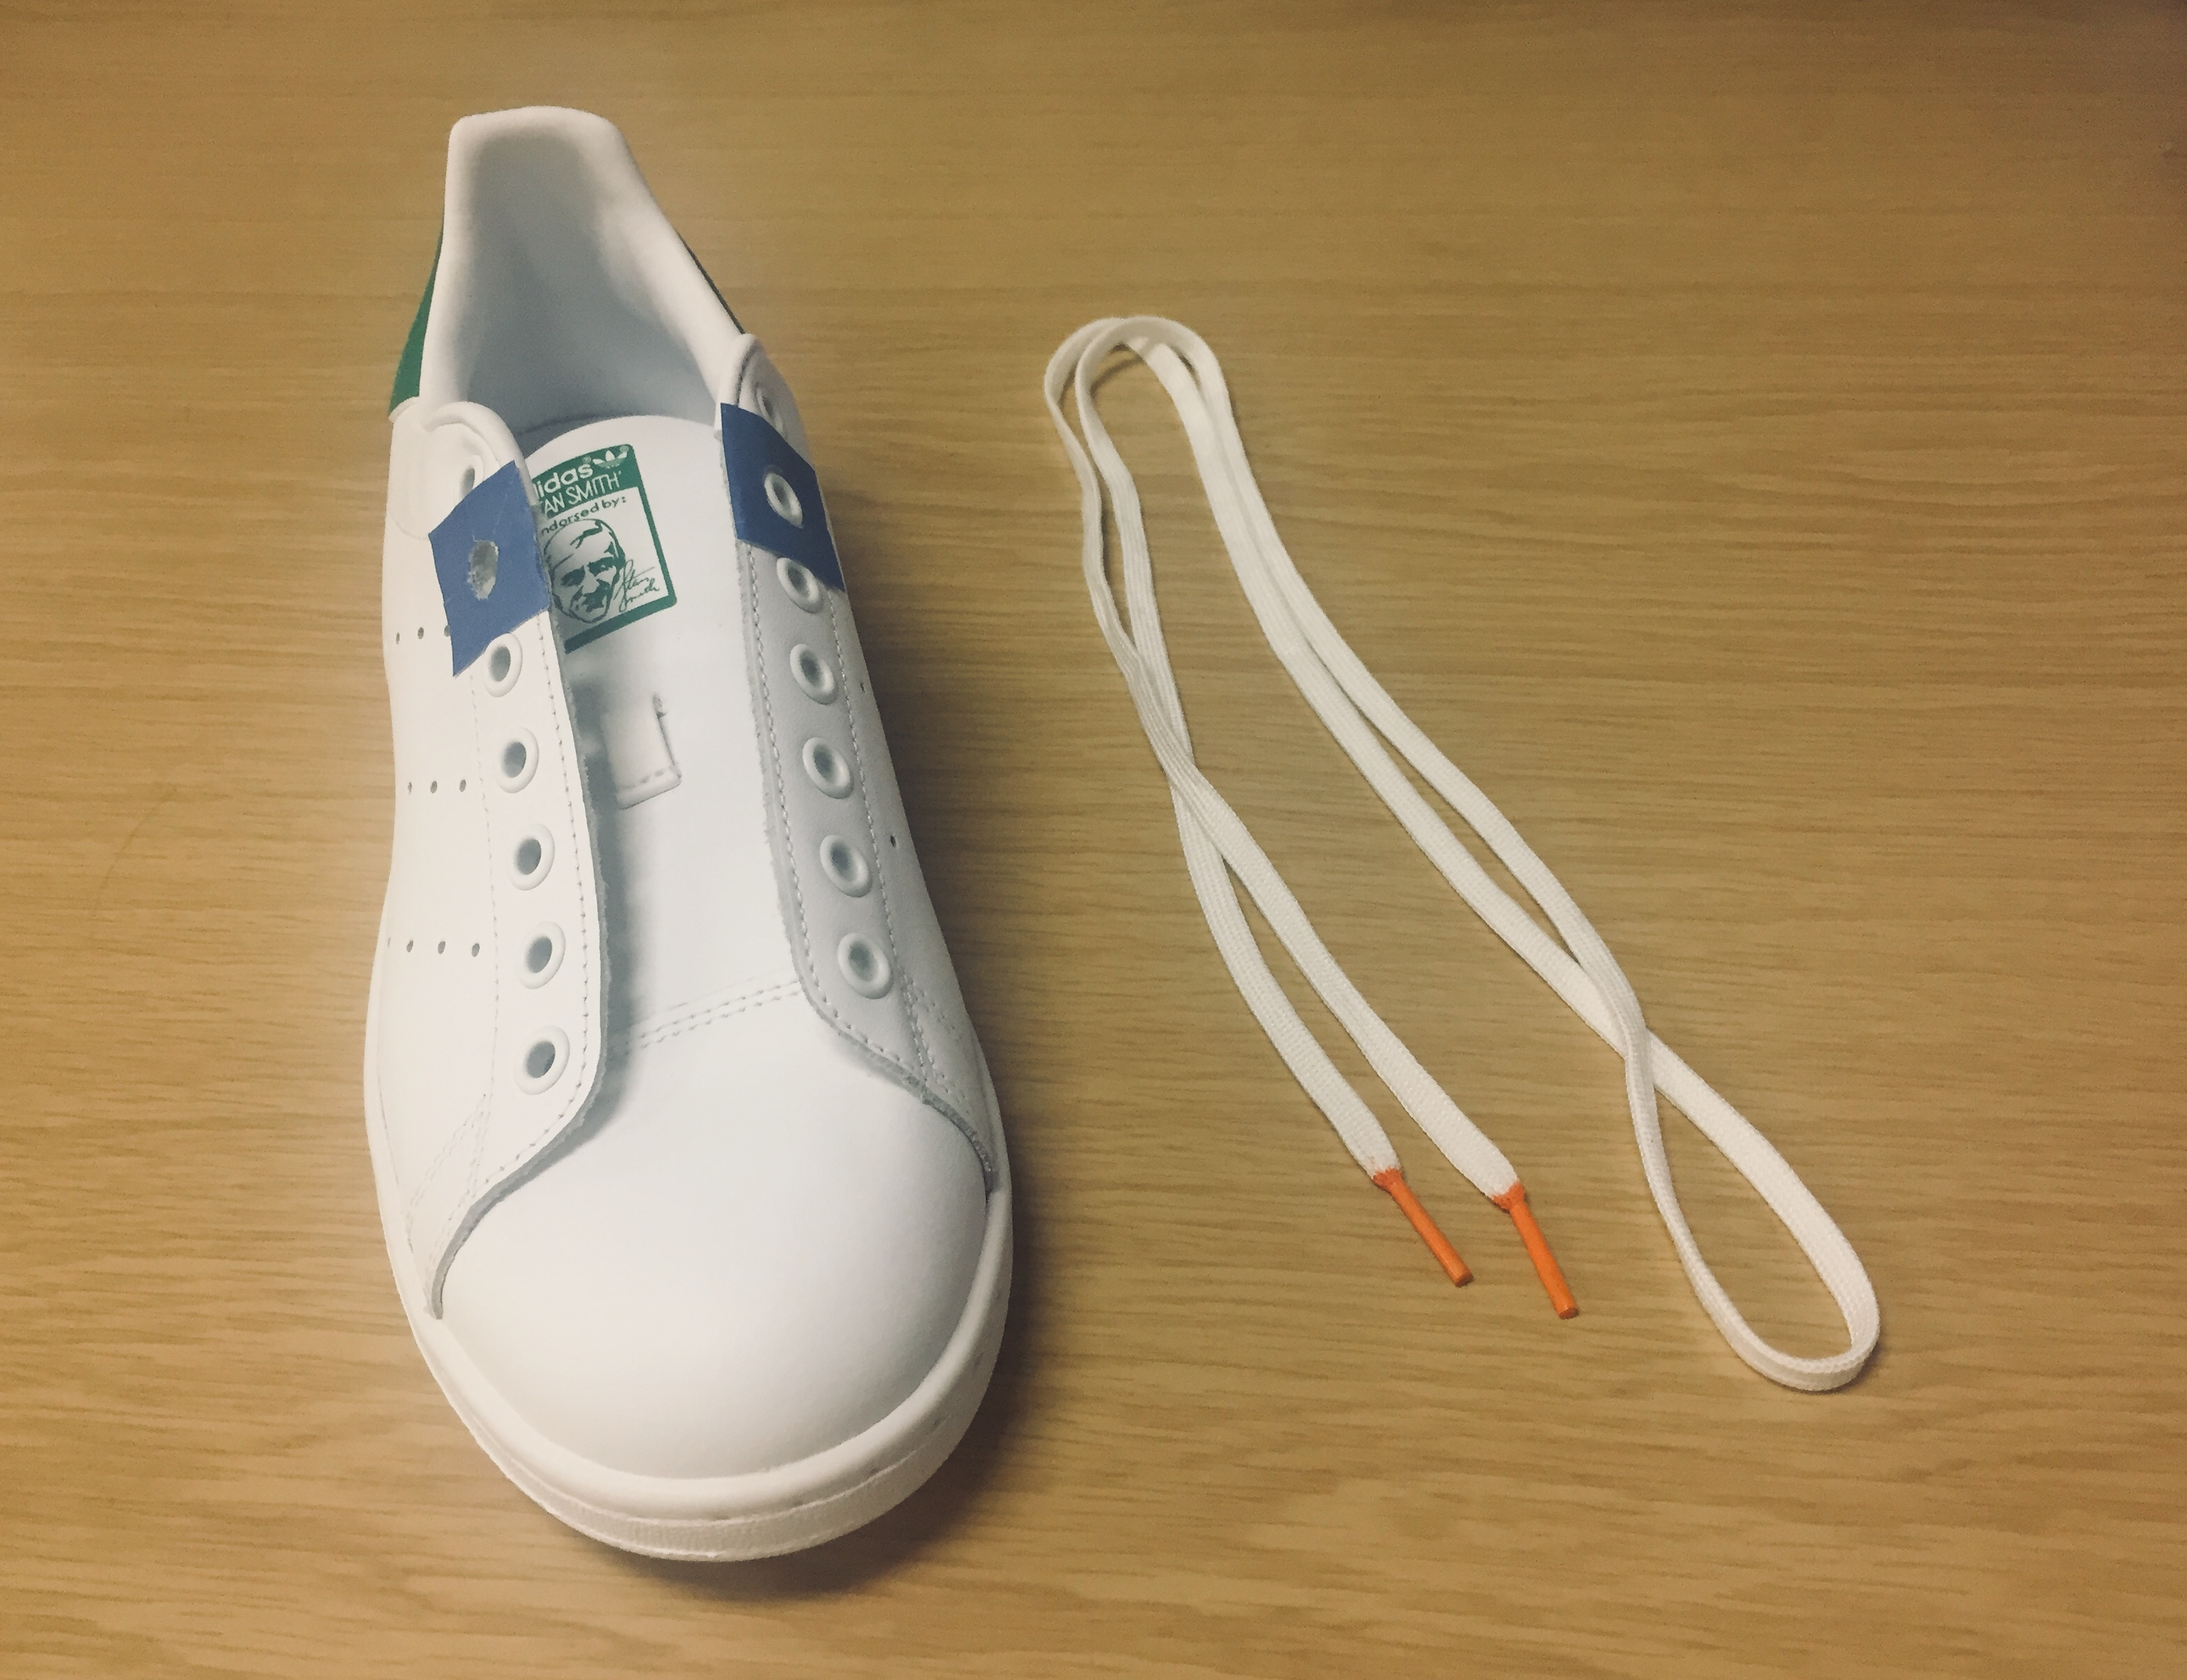
\includegraphics[width = 0.5\columnwidth]{RequirementsCap/shoe.jpg}
\caption{The manipulated shoe with distinct lace and hole colors}
\label{shoe}
\end{figure}

As illustrated in Figure \ref{shoe}, the marked shoe for manipulation has distinct colors, with orange heads of shoelace and blue shoe holes. In addition, the entire manipulation process will be carried out on the workbench of the Imperial College Personal Robotics Lab under normal lighting condition.

The project deliverables contain both core project and extensions can be divided into two main parts: Computer Vision and Motion Planning.

\section{Computer Vision}
The main aim of this part is to compute the real-time 6D pose of a specific shoe hole. There are also other tasks include providing the YuMi end-effector with the positional information needed for shoe pose adjustment, calculating the shoelace orientation before entering the second hole, etc. The algorithm must provide an accurate and stable result so that it can be used for actual shoe lace manipulation. The following features should be delivered:

\begin{itemize}
    \item \textbf{Camera Setup (core project):} Setting up the working environment for two cameras and YuMi, measuring the pose relationships between them, and installing camera dependency packages.
    \item \textbf{Shoe Detection:} Detecting the 2D bounding box of the shoe when it is placing on the workbench.
    \item \textbf{Required Locations for Shoe Pose Adjustment (extension):} Computing a series of 3D locations required by YuMi in order for it to adjust the pose of the shoe.
    \item \textbf{3D Location of Shoe Hole (core project):} Computing the 3D real-world location of the centroid of target shoe hole.
    \item \textbf{3D Orientation of Shoe Hole (core project):} Computing the 3D orientation of that hole.
    \item \textbf{6D Pose of Shoelace after Pulling (extension):} Computing the 6D pose of the shoelace after pulling it out from the first shoe hole, in order to let another gripper align with and re-clamp it before inserting the next hole.
\end{itemize}


\section{Motion Planning}
This section focus on real-world motion planning of YuMi's arms. The outcome of this part should enable YuMi to adjust the orientation of the shoe if necessary, and then put shoe lace into a hole accurately while avoiding any collisions with obstacles. Finally, YuMi should pull the shoelace out to complete that hole and adjust the gripper pose to align with the shoelace and reclamp it. So that YuMi can start to plan trajectories for next shoe hole. These objectives can be divided into following tasks:

\begin{itemize}
    \item \textbf{MoveIt! Interface and Planning Scene Setup (core project):} Setting up the MoveIt! Python interface, and initializing the manipulating environment by defining known obstacles' dimension and position.
    \item \textbf{Movement Control (core project):} Setting up the control interface among my control instructions and YuMi's grippers and arms.
    \item \textbf{Safe Positions Calculation (core project):} Calculating several safe poses of YuMi's arms, including cal pose, home pose and initial pose.
    \item \textbf{Shoe Pose Adjustment (extension):} Adjusting the orientation of shoe using YuMi gripper if its pose is not ideal. 
    \item \textbf{Robot Gripper Approaching Pose (core project):} Computing the 6D approaching pose to the interested shoe hole, and defining a series of required waypoints.
    \item \textbf{Offset Adjustment and Shoelace Insertion (core project):} Adjusting the offset between camera readings and YuMi movement, especially offset introduced by the gripper's pose, and finally inserting the shoelace into the shoe hole.
    \item \textbf{Shoelace Grabbing (extension):} Computing the 6D shoelace grasping pose in order to pull it out, and a series of motions in preparation for calculating the 6D pose of shoelace.
\end{itemize}



%\section{Testing Environment}
%light pose robot .....